\documentclass{article}
\usepackage[left=2cm,right=2cm,top=2cm,bottom=2cm]{geometry}
\usepackage[utf8]{inputenc}
\usepackage[german]{babel}
\usepackage{amsmath}
\usepackage{dsfont}
\usepackage[export]{adjustbox}
\usepackage{amsthm}
\usepackage{color}
\usepackage{amsfonts}
\usepackage{amssymb}
\usepackage{wasysym}
\usepackage{makeidx}
\usepackage{graphicx}
\usepackage[colorlinks=true,urlcolor=blue,linkcolor=blue]{hyperref}
\usepackage{ziffer}
\usepackage{minted}
\usepackage{xcolor}
\usepackage{framed}
\usepackage{mdframed}
\usepackage{subfiles}
\usemintedstyle{emacs}

\definecolor{purp}{HTML}{9A72AC}
\definecolor{re}{HTML}{FC6255}
\definecolor{gre}{HTML}{83C167}
\definecolor{blu}{HTML}{58C4DD}
\definecolor{shadecolor}{rgb}{0.85,0.85,0.85}
\definecolor{bg}{rgb}{0.95,0.95,0.95}
\setlength{\parindent}{0em} 

\BeforeBeginEnvironment{minted}{\begin{mdframed}[linewidth =2 ,backgroundcolor=bg , linecolor=black, linewidth=0.5]}
\AfterEndEnvironment{minted}{\end{mdframed}}

\newtheorem{defi}{Definition}
\BeforeBeginEnvironment{defi}{\begin{mdframed}[linewidth =2 ,backgroundcolor=bg , linecolor=black, linewidth=0.5]}
\AfterEndEnvironment{defi}{\end{mdframed}}

\newcommand{\bsp}{\textbf{Beispiel}:}
%\newcommand{\task}{\textbf{Aufgabe}:}

\newcommand{\bol}[1]{\textbf{#1}}
\newcommand{\q}[1]{\glqq #1\grqq}
\newcommand{\DODO}[1]{\textbf{\textcolor{red}{DODO:}} #1 \\ \begin{center}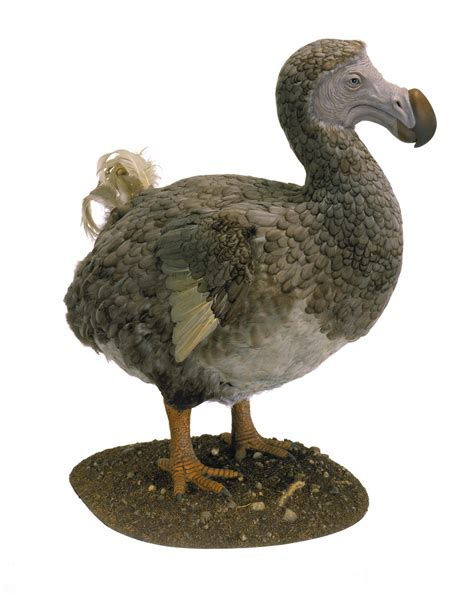
\includegraphics[scale=0.2]{../../media/dodo.jpg} \end{center}}

\newenvironment{task}[1]{
    \begin{shaded*}
    \textbf{Aufgabe #1}:
}{
    \end{shaded*}
}



\begin{document}
\subsection{Die $\mathcal{O}$ - Notation}
Grundsätzlich geht es bei der $\mathcal{O}-$ Notation darum, wie der Ressourcenbedarf unserer Algorithmus für große Eingaben skaliert (dabei kann sowohl die Laufzeit, als auch der Speicherplatzbedarf betrachtet werden). Explizit \textbf{nicht} betrachtet werden:
\begin{itemize}
    \item Programmiersprache
    \item Betriebssystem
    \item Prozessorleistung
    \item Speicherausstattung
    \item Computerarchitektur
    \item etc. 
\end{itemize}
Es geht rein um die Effizienz des Algorithmuses, nicht um seine konkrete Umsetzung auf einer bestimmten Hardware. Ist der Algorithmus zu \q{schlecht}, so ist er ggf. auf keiner Hardware praktisch umsetzbar!
\begin{center}
    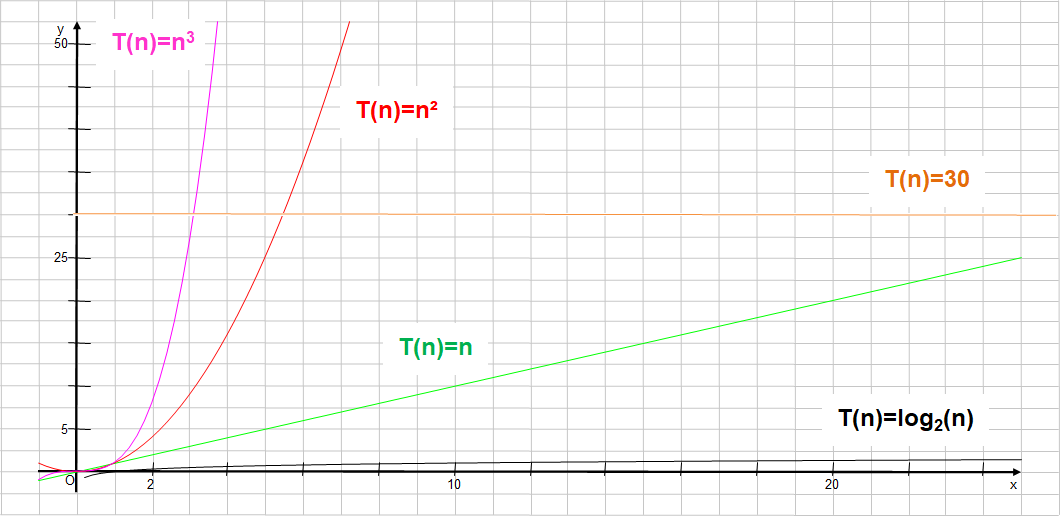
\includegraphics[scale=0.55]{../media/o.png}
\end{center}
Bei der Analyse eines Algorithmuses geht es in der Regel darum, eine \textbf{worst-case} oder \textbf{average-case}- Abschätzung zu machen. Wir beschränken uns auf den ersten Fall. \\
Grob gesprochen ist das Ziel, eine Funktion zu finden, die das Wachstum unserer Laufzeit nach oben begrenzen. Die Laufvariable der Funktion entspricht dabei in der Regel der Länge (oder Größe) der Eingabe. \\
Der Parameter $n$ der Funktion oben könnte zum Beispiel für die Länge eines Strings stehen, oder für die Einträge eines Arrays. Wir wollen wissen, welche Art von Funktion als obere Grenze geeignet ist. \\
Natürlich sollte die Funktion dafür möglichst wenig \q{wachsen}. Am Besten ist demzufolge eine konstante Laufzeit (im Beispiel oben $T(n)=30$), denn hier ist die Länge überhaupt nicht relevant! \\
\textbf{Noch einmal als wichtiger Hinweis:} es geht uns hier jetzt nicht um eine exakte Anzahl an Operationen, oder eine exakte Laufzeit, sondern nur ein \textbf{asymptotisches} Verhalten!  \\
Einige grundlegende Abschätzungen:
\begin{itemize}
    \item \q{einfache} Operationen wie das Verrechnen von Zahlen, das Prüfen einer Bedingung, eine Zuweisung, etc. haben eine konstante Laufzeit. 
    \item Ist eine Wiederholung im Spiel (z.B. for $i = 0$ to $n$), dann liefert uns dies eine lineare Laufzeit $T(n) = n$.
    \item Auch wenn die Wiederholung nur bis z.B. $\frac{n}{2}$ läuft spricht man von linearer Laufzeit, mathematisch: multiplikative Konstanten spielen keine Rolle, d.h. $n$ ist eine genauso \q{gute} Laufzeit wie $10000n$, da das Wachstum immer noch linear ist.
    \item Werden Wiederholungen ineinander geschachtelt, so erhält man höhere Polynome als Laufzeit, da beispielsweise für jeden einzelnen Listeneintrag die gesamte Liste wieder durchlaufen wird (das ergibt $n^2$), usw. 
    \item Im Falle unseres Baumes kommt es häufig zu logarithmischen Laufzeiten (dem Besten Fall außerhalb der konstanten Laufzeit). Der Logarithmus ist bekanntlich die Umkehrung der Potenz, d.h.: halbiert sich die Problemgröße in jedem Schritt (z.B. durch Auswahl des linken oder rechten Teilbaums), so ergibt sich eine Laufzeit von $log_2(n)$.  
\end{itemize}
Ein Beispiel:
\begin{minted}{Java}
    int sum = 0;
    for(int i = 0; i < n; i++) {
        for(int j = 0; j < n/2; i++) {
            summe += 1;
        }
    }
    for(int k = 0; k < n; k++) {
        sum -= 1;
    }
\end{minted}
Im ersten Block gibt es zwei ineinandergeschachtelte Wiederholungen, d.h. das inkrementieren wird $n \cdot \frac{n}{2} = \frac{1}{2} n^2$ mal ausgeführt. In der zweiten Wiederholung gibt es dagegen $n$ Ausführungen. Damit insgesamt:
\begin{center}
    $\frac{1}{2} n^2 + n$
\end{center}
Operationen. Konstante multiplikative Faktoren spielen keine Rolle, ebensowenig wie das $n$ - denn für $n\rightarrow \infty$ wächst das Quadrat viel stärker als der lineare Summand. Man würde deswegen für diesen Algorithmus folgern:
\begin{center}
    $\mathcal{O}(n^2)$
\end{center}
Der Algorithmus verhält sich für große $n$ also näherungsweise quadratisch. \\
Weitere Details: siehe Studium bzw. 12. Klasse!
\end{document}